\chapter{Minimal problems in computer vision geometry}\labelcha{app}
Many problems from computer vision geometry can be modeled by systems of polynomial equations.
A problem that requires only the minimal subset of data points to solve the problem is called a minimal problem.
A typical example is the 5-point algorithm \cite{5pt} for relative pose estimation between two cameras given five image correspondences only.
In many applications, solvers of these minimal problems are used in the Random Sample Consensus (RANSAC) algorithm \cite{ransac}, where the minimal problems has to solved repeatedly for a large amount of input data.
Thus, these solvers are required to be fast and efficient.
The state of the art method is to generate these solvers by automatic generators \cite{autogen}, which are based on Gr\"obner basis construction and eigenvectos of multiplication matrices computation.
In these solvers both real and non-real are computed, but the non-real solutions are discarded, since they have no geometric meaning.

In \refsec{POP:sol}, we have proposed and implemented an algorithm, which does not need to compute the superfluous non-real solutions, and therefore may be faster than the standard solvers generated by the automatic generators.
In this section, we compare the speed and numerical stability of the state of the art solvers with our implementation of the moment method algorithm for polynomial system solving.
For this reason, we have selected few minimal problems from computer vision geometry, on which we will compare the selected solvers.

\section{Dataset description}
\input{macros/app_LADIO.tex}
First of all, we describe the scene, which we have chosen for our experiments.
It is a real scene of a sculpture of Buddha head taken for the LADIO \cite{ladio} experiments.
%TODO: cite Ladio experiments
The reconstructed surface of the sculpture can be seen in \reffig{app:LADIO}.
There are \importAppLADIONumCameras{} taken images of the sculpture, from which \importAppLADIONumPoints{} 3D points were reconstructed using a scene reconstruction pipeline including ...
%TODO: fill missing part of the pipeline

\begin{figure}[ht]
  \centering
  \begin{subfigure}[b]{0.45\textwidth}
    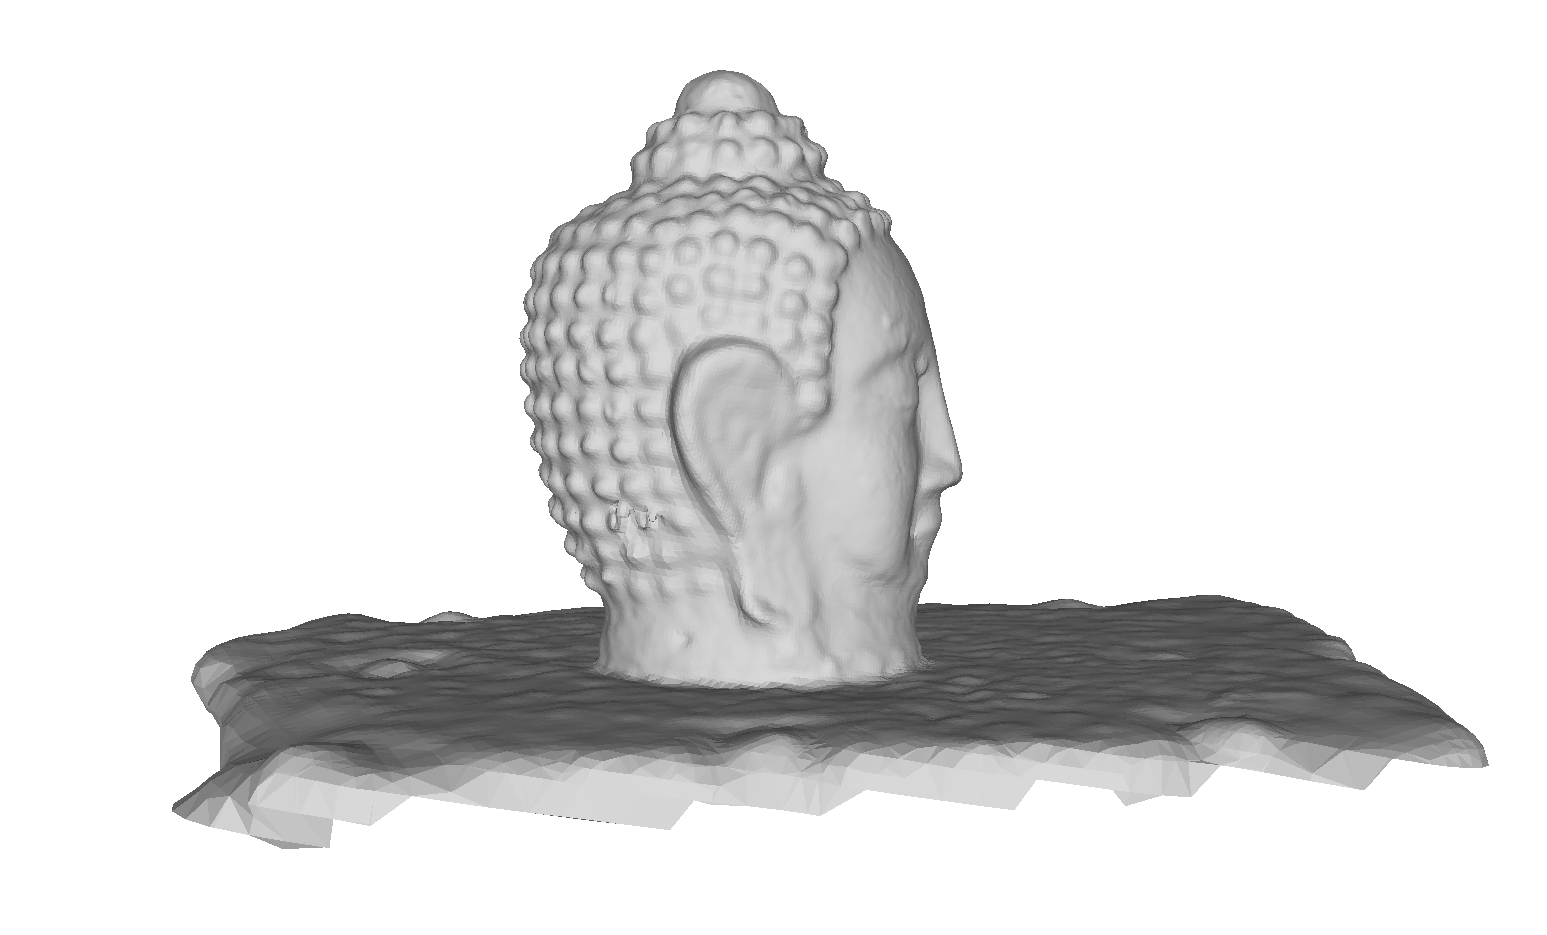
\includegraphics[width=0.95\textwidth]{images/LADIO_01.png}
    \vspace{2mm}
  \end{subfigure}
  ~
  \begin{subfigure}[b]{0.45\textwidth}
    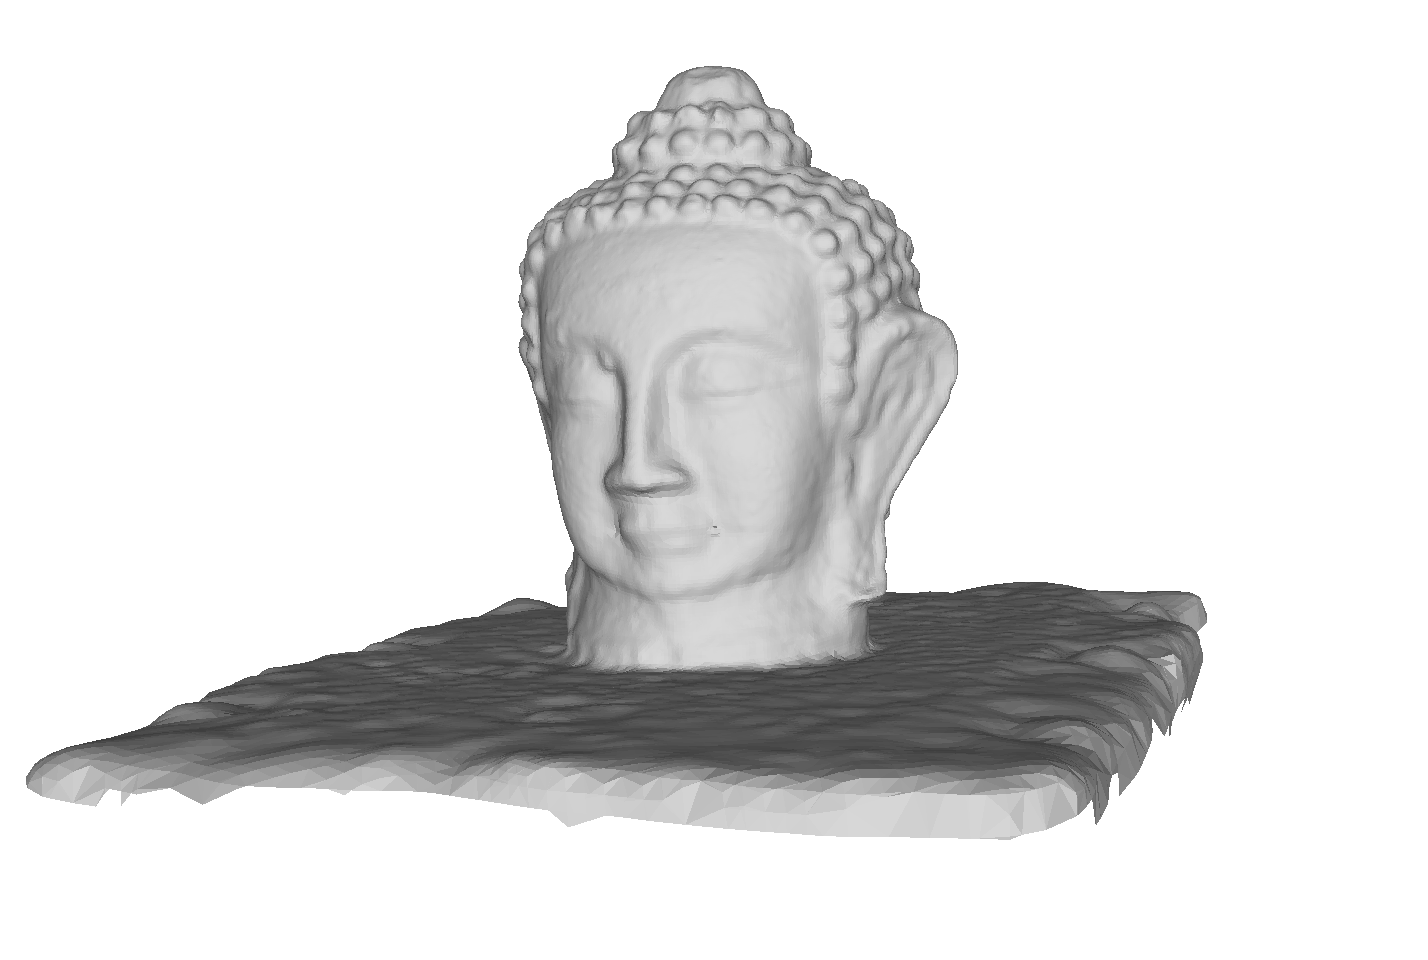
\includegraphics[width=0.90\textwidth]{images/LADIO_02.png}
  \end{subfigure}
  \caption{Sculpture of Buddha head. Surface representing a point cloud reconstructed from the taken images.}
  \labelfig{app:LADIO}
\end{figure}

\section{Calibrated camera pose}
Computation of calibrated camera pose (its rotation and location with respect to the global coordinate system) is one of the typical problems in computer vision.
The pose can be computed from at least three known 3D points and their perspective projection into the image plane, thus the problem is called the perspective-three-point (P3P) problem and it is known since 1841 from \cite{p3p1841}, but its modern and complete description can be found in \cite{P3P}.

\begin{figure}[ht]
  \centering
  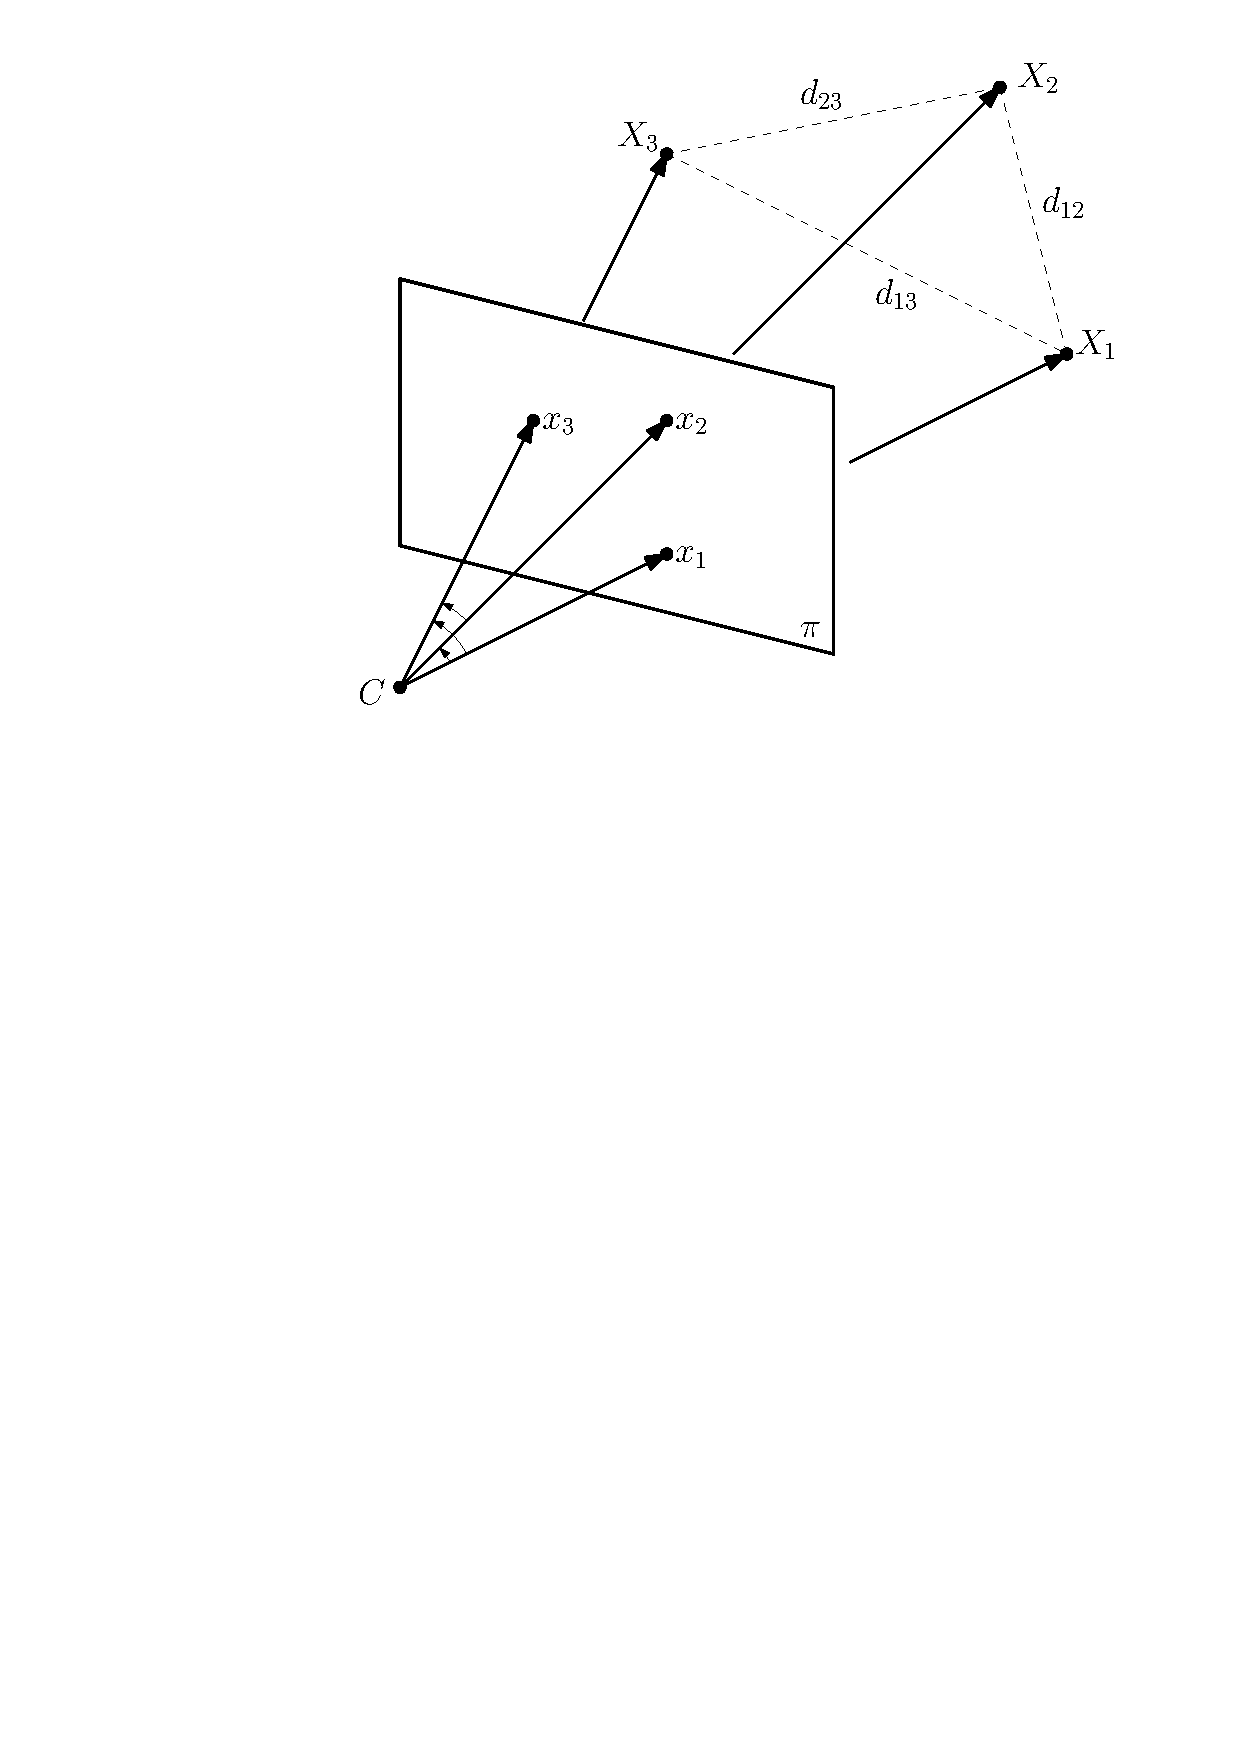
\includegraphics[width=0.5\textwidth]{drawings/P3P.pdf}
  \caption{Scheme of the P3P problem. A pose of a calibrated camera can be computed from three known 3D points $X_1$, $X_2$, $X_3$ and their projections $x_1$, $x_2$, $x_3$ into the image plane $\pi$. The camera projection center is denoted as $C$. Distances $d_{12}$, $d_{23}$, $d_{13}$ denote the distances between the respective 3D points.}
  \labelfig{app:P3P}
\end{figure}

The problem is stated followingly:
Given three 3D points $X_1, X_2, X_3 \in\R^3$ in the global coordinate system and their projections $x_1, x_2, x_3 \in\R^2$ respectively into the image plane in the image coordinate system, we are looking for a camera projection center position $C\in\R^3$ and a camera rotation matrix $R\in\SO$ -- all rotations in 3D space around the origin, such that the projection equation
\begin{align}
  \lambda_i\bmB x_i\\1\bmE &= K\bmB R & -RC\bmE\bmB X_i\\1\bmE
\end{align}
holds for $i=1,2,3$ and $\lambda_i\in\R/\{0\}$, where $K\in\R^{3\times3}$ is known calibration matrix of the camera.
The situation is depicted in \reffig{app:P3P}.

It has been shown that for general case this problem can be solved by finding roots of a quartic equation in variable $\xi\in\R$
\begin{align}
  a_4\xi^4 + a_3\xi^3 + a_2\xi^2 + a_1\xi + a_0 &= 0\labeleq{app:P3P:4}
\end{align}
for coefficients $a_0, \ldots, a_4\in\R$, which can be computed by the formulae below.
\begin{align}
  a_4 &= -4d_{23}^4d_{12}^2d_{13}^2c_{23}^2+d_{23}^8-2d_{23}^6d_{12}^2-2d_{23}^6d_{13}^2+d_{23}^4d_{12}^4+2d_{23}^4d_{12}^2d_{13}^2+d_{23}^4d_{13}^4\\
  a_3 &= 8d_{23}^4d_{12}^2d_{13}^2c_{12}c_{23}^2+4d_{23}^6d_{12}^2c_{13}c_{23}-4d_{23}^4d_{12}^4c_{13}c_{23}+4d_{23}^4d_{12}^2d_{13}^2c_{13}c_{23}\\
      &-4d_{23}^8c_{12}+4d_{23}^6d_{12}^2c_{12}+8d_{23}^6d_{13}^2c_{12}-4d_{23}^4d_{12}^2d_{13}^2c_{12}-4d_{23}^4d_{13}^4c_{12}\nonumber\\
  a_2 &= -8d_{23}^6d_{12}^2c_{13}c_{12}c_{23}-8d_{23}^4d_{12}^2d_{13}^2c_{13}c_{12}c_{23}+4d_{23}^8c_{12}^2-4d_{23}^6d_{12}^2c_{13}^2\\
      &-8d_{23}^6d_{13}^2c_{12}^2+4d_{23}^4d_{12}^4c_{13}^2+4d_{23}^4d_{12}^4c_{23}^2-4d_{23}^4d_{12}^2d_{13}^2c_{23}^2+4d_{23}^4d_{13}^4c_{12}^2+2d_{23}^8\nonumber\\
      &-4d_{23}^6d_{13}^2-2d_{23}^4d_{12}^4+2d_{23}^4d_{13}^4\nonumber\\
  a_1 &= 8d_{23}^6d_{12}^2c_{13}^2c_{12}+4d_{23}^6d_{12}^2c_{13}c_{23}-4d_{23}^4d_{12}^4c_{13}c_{23}+4d_{23}^4d_{12}^2d_{13}^2c_{13}c_{23}-4d_{23}^8c_{12}\\
      &-4d_{23}^6d_{12}^2c_{12}+8d_{23}^6d_{13}^2c_{12}+4d_{23}^4d_{12}^2d_{13}^2c_{12}-4d_{23}^4d_{13}^4c_{12}\nonumber\\
  a_0 &= -4d_{23}^6d_{12}^2c_{13}^2+d_{23}^8-2d_{23}^4d_{12}^2d_{13}^2+2d_{23}^6d_{12}^2+d_{23}^4d_{13}^4+d_{23}^4d_{12}^4-2d_{23}^6d_{13}^2
\end{align}
Where the distances $d_{12}$, $d_{23}$ and $d_{13}$ are
\begin{align}
  d_{12} &= \|X_1 - X_2\|,\\
  d_{23} &= \|X_2 - X_3\|,\\
  d_{13} &= \|X_1 - X_3\|
\end{align}
and the coefficients $c_{12}$, $c_{23}$ and $c_{13}$ are cosines of angles between respective projection rays, and they can be directly computed from the projected points coordinates.
\begin{align}
  c_{12} &= \frac{x_1^\top K^{-\top} K^{-1}x_2}{\|K^{-1}x_1\|\|K^{-1}x_2\|}\\
  c_{23} &= \frac{x_2^\top K^{-\top} K^{-1}x_3}{\|K^{-1}x_2\|\|K^{-1}x_3\|}\\
  c_{13} &= \frac{x_1^\top K^{-\top} K^{-1}x_3}{\|K^{-1}x_1\|\|K^{-1}x_3\|}
\end{align}

The equation \refeqb{app:P3P:4} may have zero, two or four real roots, but some of them are discarded by checking three polynomial equations, that the law of cosines has to hold up to some numerical precision in triangles $\triangle\big(CX_iX_j\big)$ for $i,j=1,2,3$ and $i\neq j$, i.e.
\begin{align}
  d_{12}^2 &= \|X_1-C\|^2 + \|X_2-C\|^2 - 2c_{12}\|X_1-C\|\|X_2-C\|,\\
  d_{23}^2 &= \|X_2-C\|^2 + \|X_3-C\|^2 - 2c_{23}\|X_2-C\|\|X_3-C\|,\\
  d_{13}^2 &= \|X_1-C\|^2 + \|X_3-C\|^2 - 2c_{13}\|X_1-C\|\|X_3-C\|.
\end{align}
The camera pose ($C$ and $R$) is computed from each of the remaining solutions.

The P3P problem is probably the simplest problem, which could be chosen from the computer vision geometry for comparison of the polynomial systems solvers, since only one polynomial of degree four in one variable is given.
